		\chapter {Definitionen zu Strom}
Strom\index{Strom} kann dann fließen, wenn ein geschlossener \textbf{\textit{Stromkreis}}\index{Stromkreis} vorliegt. Dabei transportieren Elektronen (\(e^{-}\)) elektrische Energie von einer \textit{Strom-} bzw. \textit{Spannungsquelle} zu einem Verbraucher, der sie dann in andere Energieformen umsetzen kann. 

\subsubsection{Spannung: } \index{Spannung}
Ein Maß dafür, wie Viel Energie ein einzelnes Elektron dabei transportiert ist die Spannung \(U\) in Volt \(V\)
	\begin{equation}
	U = \frac{W}{Q} ~~~~~~~~~~~~~~ [U]=\frac{J}{C}=V
	\label{def_U}
	\end{equation}
mit \(W\) als transportierter Energie in Joule \(J\) und \(Q\) als bewegter Ladung in Coulomb \(C\).

\subsubsection{Potential: } Eigentlich handelt es sich bei Spannung um eine \textit{Potentialdifferenz}\index{Potential}\index{Spannung}. Jeder Punkt in einem Elektrischen Stromkreis hat ein Potential \(\varphi\). Es stellt dar, wie viel Energie pro Ladung frei wird, wenn zwischen einem Punkt \(P_1\) (einem beliebigen Punkt) und \(P_0\) (der Erdung\index{Erdung}\footnote{Statt der Erdung kann auch ein anderer, beliebiger Punkt \(P_0\) im Stromkreis gewählt werden, solange es immer der selbe Punkt ist.}) eine Leitung hergestellt wird. Das Potential bezeichnet man dann mit \(\varphi_{01}\). Ein weiterer Punkt \(P_2\) hat nun ein Potential \(\varphi_{02}\) in Bezug auf die Erdung und ein Potential \(\varphi_{12}\) im Bezug auf Punkt \(P_1\). \(\varphi_{12}\) bezeichnet man auch als \textit{Spannung} zwischen \(P_1\) und \(P_2\). Es gilt also:
	\begin{equation}
	U_{A~zu~B} = \varphi_{A~zu~Erdung} - \varphi_{B~zu~Erdung} = \Delta\varphi
	\label{def_potential}
	\end{equation}
Sowohl das Potential \(\varphi\), als auch die Spannung \(U\) haben die Einheit Volt \(V\).\index{Volt}

\subsubsection{Stromstärke: }
Ein Maß dafür, wie viele Elektronen in einer bestimmten Zeit durch den Stromkreis fließen ist die Stromstärke \(I\) in Ampère \(A\)\index{Stromstärke}\index{Ampère}
	\begin{equation}
	I = \frac{Q}{t} ~~~~~~~~~~~~~~ [I]=\frac{C}{s}
	\label{def_I}
	\end{equation}
mit \(t\) als Zeit in Sekunden \(s\).

\subsubsection{Leistung: }\index{Leistung!Elektrische}
Kombiniert man Spannung und Stromstärke (also Gleichungen (\ref{def_U}) und (\ref{def_I})), so kann man die Elekrtische Leistung \(P\) in Watt \(W\) errechnen: 
	\begin{equation}
	P = I \cdot U = \frac{W}{Q} \cdot \frac{Q}{t} = \frac{W}{t} ~~~~~~~~~~~~~~ [P] = \frac{J}{s}=W
	\label{def_P}
	\end{equation}
	
	
		\chapter{Widerstand}
		
		%\begin{wrapfigure}{r}{0.4\textwidth}
		\begin{figure}
		\centering
		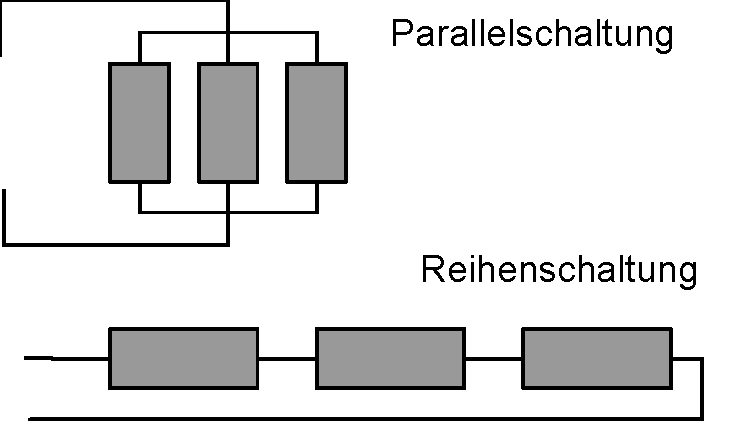
\includegraphics[width=0.6\textwidth]{mat/schaltungen}
		\caption{Arten von Schalverbänden}
		\label{img_schaltungen}
		%\end{wrapfigure}
		\end{figure}
		
Ein Widerstand\index{Widerstand!Elektrischer} ist ein technisches Bauteil, das elektrische Energie in Wärmeenergie unsetzt. In einen Stromkreis eingebaut sorgt es dafür, dass ein Teil der von der Quelle abgegebenen Leistung für einen Verbraucher nicht nurzbar ist, da sie schon vorher am Widerstand in Wärme umgesetzt wurde.\footnote{Im weitesten Sinne ist jeder nicht supraleitende Leiter ein Widerstand}

Man unterscheidet zwischen \textit{parallel} und \textit{in Reihe}\index{Parallelschaltung}\index{Reihenschaltung} geschalteten Widerständen (siehe Abb. \ref{img_schaltungen} auf S. \pageref{img_schaltungen}). Während ein Widerstand, der parallel zu einem Verbraucher geschaltet ist, die selbe Spannung \(U\) abbekommt wie der Verbraucher, wird ein Widerstand, der in Reihe zum Verbraucher geschaltet wird von dem selben Strom\footnote{also der selbe Stromstärke \(I\)} durchflossen.

Für Ohmsche Widerstände gilt dabei das \textsc{Ohm}'sche Gesetz:\index{Ohm'sches Gesetz}
	\begin{equation}
	R = \frac{U}{I} = \frac{\frac{W}{Q}}{\frac{Q}{t}} = \frac{W \cdot t}{Q^2} ~~~~~~~~~~~~~~ [R] = \frac{\frac{W}{Q}}{\frac{Q}{t}} = \frac{J \cdot s}{C^2} = \Omega
	\label{def_R}
	\end{equation}
Es besagt, dass bei sogenannten \textit{ohmschen} Widerständen\index{Widerstand!Ohm'scher} sich Stromstärke zur Spannung am Widerstand bzw. Leiter proportional zueinander verhalten. Die Proportionalitätskonstannte \(R\) stellt den Widerstand in Ohm \(\Omega\) dar. 

Aus einem Verbund an Widerständen lässt sich ein \textit{Ersatzwiderstand}\index{Ersatzwiderstand} \(R_{ersatz}\) berechnen. Man kann sich dabei vorstellen, dass man die Widerstände, die man zu seiner Berechnung heranziehr, entfernt, und dafür ein Bauteil einsetzt, das den Widerstand hat, wie die einzelnen Bauteile zusammen. Dabei muss man bei der Summation der Widerstände berücksichtigen, ob sie in Reihe oder parallel geschaltet sind; Für den Ersatzwiderstand in einer Reihenschaltung ergibt sich:
	\begin{equation}
	R_{Ersatz} = R_1 + R_2 + R_3 + ...
	\label{Rers_reihe}
	\end{equation}
Für parallel geschaltete Widerstände ergibt sich jedoch:
	\begin{equation}
	R_{Ersatz} = \frac{1}{\frac{1}{R_1} + \frac{1}{R_2} + \frac{1}{R_3} + ....}
	\label{Rers_parallel}
	\end{equation}	


%		\part{das Elekrtische Feld "`\textit{E-Feld}"'}	

		\chapter{Feldlinienmodell}

Zwischen zwei Ladungen \(Q_1\) und \(Q_2\) besteht immer ein E-Feld. Deshalb bezeichnet man sie als \textit{felderzeugende Ladungen}.\footnote{Felderzeugende Ladungen erhalten ein großes \(Q\), Probeladungen (die kleiner sind als die felderzeugenden) erhalten ein kleines \(q\).}\index{Felderzeugende Ladung}\index{Feldlinien}

Ein E-Feld ist derjenige Bereich, in dem auf ein elektrisch geladenes Teilchen -- mit der Probeladung\index{Probeladung} \(q\)  (positiv oder negativ) -- eine elektrische Kraft ausgeübt wird, die von Anziehungen oder Abstoßungen der felderzeugenden Ladungen herrühren.

Aufgrund des E-Feldes führt eine Probeladung folglich Bewegungen innerhalb des Feldes aus. Bahnen, auf denen sich eine solche Probeladung bewegen, bezeichnet man als \textit{Feldlinien}. In der Darstellung besteht die Konvention, dass man den Weg eines positiv geladenen Probeteilchens einträgt, also den Feldlinien mittels Pfeilspitzen die Richtung zuweist, die eine positive Ladung nehmen würde. Die Feldlinien laufen von einer positiven Felderzeugenden Ladung \(Q_1\) zu einer negativen \(Q_2\). Sie stehen jeweils auf der Oberfläche der Ladungsträger und kreuzen sich nicht. Für Darstellungen gilt, dass die Kräfte auf ein Probeteilchen umso stärker sind, je dichter die Feldlinien an dieser Stelle sind.

Es kann dazu kommen, dass E-Felder abgeschirmt werden -- beispielsweise beim \textsc{Faraday}'schen Käfig. Hier besteht innerhalb eines von Leitern eingeschlossenen Bereichs kein E-Feld, rundherum dagegen schon.

		\chapter{Elektrische Feldstärke}
		
		\section{Kraft auf Ladungsträger}
		\label{F_auf_q}
Die Kraft auf eine Probeladung wirkt tangential zu den Feldlinien. Diese Kraft \(F_{el}\) ist Proportional zu der elektrischen Ladung \(q\) des Teilchens. Verlaufen Feldlinien in einem Bereich gerade, parallel und im selben Abstand voneinander, so spricht man in diesem Bereich von einem \textit{homogenen} E-Feld\index{E-Feld!Homogenes}.\footnote{Es tritt beispielsweise (nährungsweise) zwischen zwei elektrisch gelandenen parallelen Platten auf.} In diesem ist die Elektrische Feldstärke \(\vec{E}\) konstant\footnote{in Betrag und Richtung}. \\
Normalerweise sind E-Felder \textit{inhomogen}.
	\begin{equation}
	\vec{E} = \frac{\vec{F_{el}}}{q} ~~~~~~~~~~~~~~ [\vec{E}] = \frac{N}{C} = \frac{\frac{J}{m}}{C} = \frac{V}{m}
	\label{def_E}
	\end{equation}
wobei \(\vec{E}\) die Elektrische Feldstärke des Feldes ist.


		\section{Distanzen im E-Feld}
Um Ladungen in einem homogenen E-Feld der Feldstärke \(E\) parallel zu den Feldlinien zu bewegen, benötigt\footnote{bzw. wird frei; bewegt man eine positive Ladung mit den Feldlinien, wird Energie frei -- in anderen Fällen entsprechend} 
man die Energie \(W\). Diese ist proportional zu der Strecke \(l\) parallel der Feldlinien, sowie der Ladung \(q\) des Teilchens. Es gilt dabei: 
	\begin{equation}
	W = q \cdot E \cdot l ~~~~~~~~~~~~~~ [W] = C \cdot \frac{N}{C} \cdot m = Nm = J
	\label{W_kondensator}
	\end{equation}
Benutzt man nun Formel \ref{def_U}, so gilt:
	\begin{equation}
	U = E \cdot l
	\label{U=El}
	\end{equation}
Interpretiert man das Ergebnis nach Formel \ref{def_potential}, so gilt folgendes: Zwischen den Punkten \(P_{1}\) und \(P_2\) in einem E-Feld liegt immer die Spannung \(\Delta\varphi = U_{1~zu~2} = E \cdot l\), wobei man die Strecke \(l\) nur in Richtung der Feldlinien messen muss.

Das bedeutet widerrum, dass man Ladungen problemlos senkrecht zu den Feldlinien bewegen kann. Diese Linien\footnote{bzw. im Raum diese Flächen} bezeichnet man als \textit{Äquipotentialflächen}.



		\chapter{Kondensator}

Im Grunde besteht ein \emph{Kondensator}\index{Kondensator} aus zwei Metallplatten, die durch ein \emph{Dielektrikum}\index{Dielektrikum} voneinander getrennt sind. Schließt man die Pole einer Spannungsquelle an einen Kondensator an, so wird er aufgeladen und kann elektrische Energie speichern und später wieder abgeben. Für Kondensatoren gibt es zahlreiche Aufbaumöglichkeiten.



		\section{Stärke des E-Felds im Kondensator}
Das Homogene E-Feld im Kondensator\index{E-Feld!Homogenes} kann man leicht ausrechnen. Durch Umformung von Formel \ref{U=El} kommt man für einen Kondensator, an dem die Spannung \(U\) zwischen zwei Platten, die sich im Abstand \(d\) voneinander entfernt befinden, anliegt,  auf:
	\begin{equation}
	E = \frac{U}{d}
	\label{E_kondensator}
	\end{equation}


		\section{Zusammenhang mit felderzeugenden Ladungen}	
Auf Kondensatorplatten der Fläche \(A\) sind die felderzeugenden Ladungen \(Q\) gleichmäßig auf der Außenseite verteilt\footnote{Es geht dabei um die Ladung \textit{einer} Platte}. Der Quotient \(\sigma\) gibt an, wie groß die Ladung auf einer bestimmten Fläche ist:
	\begin{equation}
	\sigma = \frac{Q}{A} ~~~~~~~~~~~~~~ [\sigma] = \frac{C}{m^2}
	\label{def_sigma}
	\end{equation}	
Diese \textit{Flächenladungsdichte} \(\sigma\) auf den Kondensatorplatten steht in direktem Zusammenhang mit der Feldstärke \(E\) zwischen den Platten. Es git nämlich:
	\begin{equation}
	E = \frac{\sigma}{\varepsilon_0 \cdot \varepsilon_r} ~~~~~~~~~~~~~~ [E] = \frac{\frac{C}{m^2}}{\frac{C}{Vm} \cdot 1} = \frac{V}{m}
	\end{equation}
Dabei ist \(\varepsilon_0\) die Elektrische Feldkonstante mit \(\varepsilon_0 \approx 8,85 \cdot 10^{-12} \frac{C}{Vm}\) und \(\varepsilon_r\) die Dielektritätszahl (\(\rightarrow\) Kapitel \ref{kap_epsilon_r})  mit \(\varepsilon_r \approx 1\) für Luft.


		\section{Kapazität}
Die Kapazität \(C\)\index{Kapazität} eines Kondensators gibt an, wie viel Ladung \(Q\) bei einer bestimmten Spanung \(U\) gespeichert werden kann. Sie ist deshalb definiert als der Quotient von Ladung \(Q\) und Spannung \(U\):
	\begin{equation}
	C = \frac{Q}{U} ~~~~~~~~~~~~~~ [C] = \frac{C}{V} = F
	\label{def_C}
	\end{equation}
Dabei ist \(C\) die Kapazität in Farad \(F\). 

Die Kapazität eines Plattenkondensators mit homogenem E-Feld kann darüber hinaus noch folgendermaßen berechnet werden:
	\begin{equation}
	C = \varepsilon_0 \cdot \varepsilon_r \cdot \frac{A}{d} ~~~~~~~~~~~~~~ [C] = \frac{C}{Vm} \cdot \frac{m^2}{m} = \frac{C}{V} = F
	\label{C_kondensator}
	\end{equation}
Wobei \(A\) die Oberfläche einer Platte in \(m^2\) und \(d\) der Abstand der Platten in \(m\) darstellt.


		\subsection{Dielektrizitätszahl}
		\label{kap_epsilon_r}
Die Dielektrizitätszahl \(\varepsilon_r\)\index{Dielektrizitätszahl} gibt an, um welchen Faktor sich die Kapazität verändert, wenn ein \textit{Dielektrikum}\footnote{Materie im Kondensator, durch die das E-Feld geht} eingeführt wird. Es handelt sich dabei um eine Materialkonstante die vom Stoff anbängt. Es gilt dabei:
	\begin{equation}
	\varepsilon_r = \frac{C_{Dielektrikum}}{C_{Vakuum}}
	\label{def_epsilon_r}
	\end{equation}
Weiter gilt als gute Nährung \(C_{Vakuum} \approx C_{Luft}\) 	


		\section{Schaltungen von Kondensatoren}
Schaltet man Kondensatoren parallel (\(\rightarrow\) Abb. \ref{img_schaltungen}), so kann man als \textit{Ersatzkapazität} die Kapazitäten der einzelnen Kondensatoren Addieren:
	\begin{equation}
	C_{Ersatz} = C_1 + C_2 + C_3 + ...
	\end{equation}
Man kann sich dabei vorstellen, das die Platten der Kondensatoren, die den selben Plattenabstand haben, seitlich aneinander angefügt werden und sich somit eine Fläche ergibt, die sich aus allen Teilflächen addiert. Betrachtet man nun Formel \ref{C_kondensator}, so ist ersichtlich, wieso man so rechnet.

Schaltet man die Kondensatoren dagegen in Reihe, so muss man zum Berechnen der Ersatzkapazität folgendermaßen vorgehen:
	\begin{equation}
	C_{Ersatz} = \frac{1}{\frac{1}{C_1} + \frac{1}{C_2} + \frac{1}{C_3} + ....}
	\end{equation}
Hierbei ist es so, als würden sich die Plattenabstände aller Kondensatoren mit den Selben Plattenflächen addieren. Aus Formel \ref{C_kondensator} ist dieses Vorgehen wieder ersichtlich.


		\section{Speichern von Energie im Kondensator}	
Ein Kondensator kann an einer Spannungsquelle aufgeladen werden. Diese kann dann abgetrennt werden. Da das E-Feld zwischen den Kondensatorplatten von den Ladungen \(Q_{1,2}\) auf den Platten kommt, und diese Ladungen nicht abfließen können, bleibt das E-Feld weiterhin erhalten. In ihm ist nun Energie gespeichert\footnote{beispielsweise kann ein geladenes Teilchen immernoch darin bewegt werden \(\rightarrow\) Formel \ref{W_kondensator} oder sie kann einen Verbraucher dazu bringen, Arbeit zu verrichten}.

Nach Formel \ref{def_U} kann man die gespeicherte Energie des Kondensators berechnen, indem man Spannung \(U\) und Ladung \(Q\) multipliziert. Da die Spannung dabei nicht konstant ist, sondern sich proportional zur Ladung verhält (\(\rightarrow\) Formel \ref{def_C}), berechnet man dazu das Integral:
	\begin{equation}
	W = \int^{U_B}_{U_A} C\cdot U ~dU = \left[ \frac{1}{2} \cdot C \cdot U^2 \right]^{U_B}_{U_A} = \frac{1}{2} \cdot C \cdot U^2_B - \frac{1}{2} \cdot C \cdot U_A^2
	\label{W_speicherung}
	\end{equation}
Das Integral ließe sich mit Formel \ref{def_C} umschreiben:
	\begin{equation}
	W = \int^{U_B}_{U_A} C\cdot U ~dU = \left[ \frac{1}{2} \cdot Q \cdot U \right]^{U_B}_{U_A}
	\end{equation}
Wird ein Dielektrikum\index{Dielektrikum} eingeführt, so erhöht sich die Speicherkapazität des Kondensators um den Faktor \(\varepsilon_r\), da sich die Kapazität ja genauso erhöht (\(\rightarrow\) Kapitel \ref{kap_epsilon_r}).


		\subsection{Energiespeicherort}
Die Energie, die der Kondensator speichert, wird in dem Raum gespeichert, den das E-Feld ausfüllt. Formel \ref{W_speicherung} kann man umformen (der Einfachheit halber sei \(U_A = 0\) und \( U_B = U\)):
	\begin{equation}
	W = \frac{1}{2} \cdot Q \cdot U = \frac{1}{2} \cdot C \cdot U^2 = \frac{1}{2} \cdot \varepsilon_0 \cdot \varepsilon_r \cdot \frac{A}{d} \cdot E^2 \cdot d^2 =  \frac{1}{2} \cdot \varepsilon_0 \cdot \varepsilon_r  \cdot E^2 \cdot V
	\end{equation}
Wobei \(V\) das Volumen des vom homogenen E-Feld durchsetzten Raum im \(m^3\) darstellt.	


		\chapter{Teilchen im E-Feld}
		
		\section{Beschleunigung}
		
		%\begin{wrapfigure}{l}{0.23\textwidth}
		\begin{figure}
		\centering
		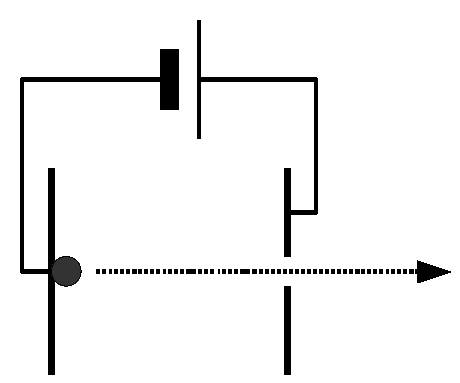
\includegraphics[width=0.6\textwidth]{mat/beschleunigung}
		\caption{negatives Teilchen beschleunigt}
		\label{img_beschleunigung}
		%\end{wrapfigure}
		\end{figure}
Ein geladenes Teilchen kann mit einem E-Feld beschleunigt werden. Aufbau siehe Abb. \ref{img_beschleunigung} auf S. \pageref{img_beschleunigung}. Dazu ist in einer der Kondensatorplatten ein Loch. Das Teilchen wird zur gegenüberliegenden Platte gebracht und diese wird gleichnamig zum Teilchen geladen -- die Platte mit Loch entsprechend ungleichnamig -- indem eine Spannung \(U\) angelegt wird.

Von der Platte ohne Loch wird das Teilchen also abgestoßen und von der mit Loch angezogen. Da das Teilchen dabei möglichst den kompletten Kondensator durchfliegt, nimmt es nach Formel \ref{def_U} die Energie \(W = U \cdot q \) auf. Diese Energie wird bei dem Teilchen vollständig in Bewegungsenergie umgewandelt und somit ergibt sich mit der Formel für kinetische Energie:
	\begin{equation}
	v = \sqrt{\frac{2 \cdot W}{m}} = \sqrt{\frac{2 \cdot U \cdot q}{m}} ~~~~~~~~~~~~~~ [v] = \sqrt{\frac{\frac{J}{C}\cdot C}{kg}} = \sqrt{\frac{Nm}{kg}} = \frac{m}{s}
	\end{equation}
Dabei ist \(m\) die Masse des Teilchens.

		\section{Ablenkung}
		\begin{figure}
		\centering
		%\begin{wrapfigure}{r}{0.23\textwidth}
		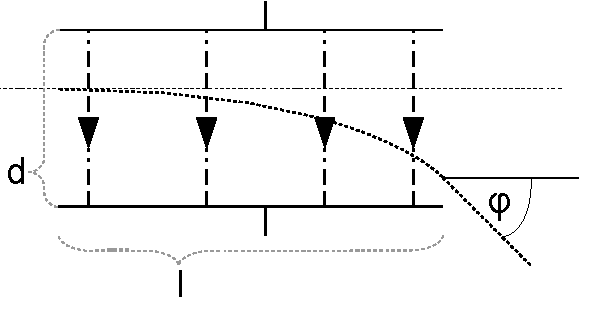
\includegraphics[width=0.6\textwidth]{mat/ablenkung}
		\caption{Teilchen wird abgelenkt}
		\label{img_ablenkung}
		%\end{wrapfigure}
		\end{figure}
Aus Kapitel \ref{F_auf_q} wissen wir, dass ein geladenes Teilchen im E-Feld eine Kraft erfährt, die von seiner Ladung abhängt (\(\rightarrow\) Formel \ref{def_E}). Bewegt sich nun ein Teilchen zwischen zwei Kondensatorplatten, zwischen denen eine Spannung \(U\) anliegt, durch, so befindet es sich in einem E-Feld, von dem es abgelenkt wird. Siehe dazu Abb. \ref{img_ablenkung} auf S. \pageref{img_ablenkung}.

Zu der anfänglichen Bewegung \(v_0\) kommt im Kondensator noch eine weitere, gleichmäßig beschleunigte Bewegung \(v_1\) -- abhängig von der Ladung \(q\) und der Masse \(m\) des Teilchens -- in Richtung einer der beiden Platten\footnote{positiv geladene Teilchen werden in Richtung der negativ geladenen Platte abgelenkt und entsprechend} hinzu. Für die Distanz \(\Delta y\), die das Teilchen in Richtung einer Platte abgelenkt wurde gilt:
	\begin{equation}
	\Delta y = \frac{E \cdot q}{2 \cdot m} \cdot t^2 = \frac{U \cdot q}{2 \cdot d \cdot m} \cdot t^2 = \frac{U \cdot q}{2\cdot d \cdot m \cdot v_0^2} \cdot ( \Delta x)^2
	\label{ablenkung_kondensator}
	\end{equation}
Dabei ist \(E\) die Feldstärke des E-Feldes zwischen den Kondensatorplatten, \(U\) die Spannung zwischen den beiden Platten, \(d\) der Abstand zwischen den beiden Platten und \(\Delta x\) die Distanz in Richtung der ursprünglichen Bewegung, die das Teilchen schon im Kondensator hinter sich gebracht hat. 

Das Teilchen folgt im Kondensator also einer Parabelförmigen Flugbahn.


		\subsection{Weiterflug}
Verlässt das Teilchen dann den Kondensator, nachdem es ihn auf der Länge \(l\) (parallel zu den Platten gemessen) durchflogen hat, so setzt sich seine Bewegung aus zwei gleichförmigen Bewegungen zusammen -- \(v_0\) und \(v_1\), da nun keine Beschleunigenden Kräfte mehr auf sie wirken. Es ergibt sich dadurch eine Gesamtgeschwindigkeit \(v_{ges}\) von:
	\begin{equation}
	v_{ges} = \sqrt{v_0^2 + v_1^2}
	\end{equation}
Mit dieser Geschwindigkeit setzt das Teilchen seinen Weg fort. Um die Richtung zu ermitteln, leitet man Formel \ref{ablenkung_kondensator} ab. Den Winkel \(\varphi\) zwischen der Neuen Flugbahn \(\vec{v}_{ges}\) und der alten \(\vec{v}_0\) erhält man mithilfe dieser Ableitung:
	\begin{equation}
	\varphi = \tan \left ( \frac{U \cdot q \cdot l}{d \cdot m \cdot v_0^2} \right )
	\end{equation}
Dabei ist \(U\) die Spannung, die zwischen den Kondensatorplatten anligt, \(m\) die Masse des Teilchens, \(q\) seine Ladung und \(v_0\) die Geschwindigkeit, mit der es parallel zu den Platten ankam.


% \part{Anhang}
%
% \chapter{Definitionen, Größen}
%
% \begin{description}
% 	\item[\(\varepsilon_0\)] Elektrische Feldkonstante \(\varepsilon_0 \approx 8,85 \cdot 10^{-12} \frac{C}{Vm}\)
% \end{description}
